\documentclass[12pt]{article}
\usepackage{epsfig,amsmath,amsthm,amssymb,amstext,vin}
\usepackage{amsthm,amsmath,amsfonts,amssymb,amscd,latexsym,txfonts}
\usepackage{mathrsfs,scalerel}
\usepackage{algpseudocode}
\usepackage{listings}
\usepackage{comment}
\pagestyle{empty}
\textheight=8.5in
\textwidth=7in
\oddsidemargin=0.0in
\begin{document}
\centerline{\Large Inverse Laplace transform and Post Inversion Formula \#7}
\vspace{1cm}

\newsavebox\foobox
\newlength{\foodim}
\newcommand{\slantbox}[2][0]{\mbox{%
        \sbox{\foobox}{#2}%
        \foodim=#1\wd\foobox
        \hskip \wd\foobox
        \hskip -0.5\foodim
        \pdfsave
        \pdfsetmatrix{1 0 #1 1}%
        \llap{\usebox{\foobox}}%
        \pdfrestore
        \hskip 0.5\foodim
}}
\def\Laplace{\ThisStyle{\slantbox[-.45]{$\SavedStyle\mathscr{L}$}}}


\section{Introduction}

Laplace transform and inverse Laplace are powerful mathematical tools. Here is the definition of Laplace transform:
$$F(s) = \int_{0}^{\8} e^{-st} f(t) dt$$

However, there is not an easy way to perform inverse Laplace transform on an arbitrary function. Fourier-integral is shown to be identical to inverse Laplace transform. However, computing a complex contour integral is nontrivial. Most of the time, we choose to match parts to known transform formula. There is no guarantee that this method will always work. A general approach to tackle inverse Laplace transform can be very valuable.
$$ \mathscr{L}^{-1}\{ F(s) \} = \frac{1}{2\pi i}\lim_{T \rightarrow \8} \int_{\lambda - i T}^{\lambda + i T} e^{s t} F(s) ds $$

This paper is dedicated to a research of general approach to find the Inverse Laplace function of any arbitrary function. Post Inversion Formula is a theoretical general approach to find the inverse Laplace transform (See section 2 for more information). \cite{PI} However, mathematicians often believe that Post Inversion Formula is too computational intensive to be put into practical usage. In this paper, however, we introduce an algorithm that compute Post Inversion Formula with power series method (See section 3 for more information). This paper also contains some example codes and algorithm analysis.

All source codes are available at 
https://github.com/fredzqmNumericInverseLaplace


\section{Post Inversion Formula}

Emil Post discovered Post's Inversion Formula, which is a simple-looking but usually impractical formula for evaluating an inverse Laplace transform. F(s) is the Laplace transform of f(t).
\begin{equation*}
f(t) = \lim_{k \rightarrow \8}\frac{(-1)^{k}}{k!} \left(\frac{k}{t}\right)^{k+1}  F^{(k)} \left(\frac{k}{t}\right)
\end{equation*}
As we can see from this formula, as k approaches infinity, we have several computational obstacles:
\begin{enumerate}
\item
	\textbf{High order of derivatives}: $F^k$ is going to be an higher order derivative of F. The traditional way to perform derivative requires high precision and division of tiny numbers. If we apply this method to a function repeatedly, the number will get distorted in the end. For many functions, as the order grows, the derivatives grow exponentially.

\item 
	\textbf{Overflow and underflow}: $\frac{1}{k!}$  is going to growing very small, while $\frac{k}{t}^{k+1}$ is growing very large. Gigantic and tiny number are both very challenge to software. The commonly used double precision floating number ranges from $2.22507*10^{-308}$ to  $1.79769*10^{308}$. Those fast growing or diminishing number exceeds this range quickly. This overflow and underflow happen when k reaches around 180.
	High-order derivative is also one source of underflow. For many functions, chain and product rules cause the derivatives to approach infinitesimal, quickly beyond the range of double precision floating number.

\item
 	\textbf{Slow convergence}: To acquire one single value, we need to perform a sequence of intensive computation to confirm the convergence. It is hard in general to know when it reaches the convergence and how accurate the result is. It is very inefficient to compute the formula above hundreds of time to get just one point in the final inverse Laplace transform curve.
\end{enumerate}

This paper will discuss the PSM method that solve the first two computational obstacles and use Post Inversion Formula to perform inverse Laplace transform. The last obstacle can be overcome with smart program that carefully selects k value and claims convergence when error is small enough.

\section{Power Series Method (PSM)}

This section will illustrate Power Series Method and how it is used to calculate the high order derivatives.
Given a differential equations system and initial conditions, Picard Iterative Process constructs a sequence of function set approaching the solution.

For instance, consider a three variable differential equation system:
\begin{equation}
\frac{dx}{dt} = f_{x}(t, x, y, z) \qquad
\frac{dy}{dt} = f_{y}(t, x, y, z) \qquad
\frac{dz}{dt} = f_{z}(t, x, y, z)
\end{equation}	
\begin{equation}
x_{0}(t) = x_{0} \qquad
y_{0}(t) = y_{0} \qquad
z_{0}(t) = z_{0}
\end{equation}
We can use the following Picard Iteration formula to generate a sequence of $x_{n}(t),y_{n}(t),z_{n}(t)$. As n grows, those function become closer to the solution of the differential system. See for example \cite{PICARD}
\begin{equation}
x_{n+1}(t) = x_{0} + \int_{t_{0}}^{t} f_{x}(t, x_{n}(t),y_{n}(t),z_{n}(t)) dt
\end{equation}
\begin{equation}
y_{n+1}(t) = y_{0} + \int_{t_{0}}^{t} f_{y}(t, x_{n}(t),y_{n}(t),z_{n}(t)) dt
\end{equation}
\begin{equation}
z_{n+1}(t) = z_{0} + \int_{t_{0}}^{t} f_{z}(t, x_{n}(t),y_{n}(t),z_{n}(t)) dt
\end{equation}
Picard iteration is widely used to solve complex differential equation system numerically. To take advantage of Picard Iteration, we have to restrict arithmetic in $f_{x,y,z}$. When these functions contain only additions and multiplications (referred as Normalized system in this paper), it has a nice property. Since $x_{0}(t),y_{0}(t),z_{0}(t)$ are constants initially, their integrals $x_{n}(t),y_{n}(y),z_{n}(t)$ are all polynomials for the solution. In that case, Picard Iterative Process generates a Taylor approximation at a given point of the function. Then, we can find the high order derivatives through those polynomials fairly quickly, see \cite{PSM}.

\subsection{Normalization of an arbitrary function}

Though Picard Iteration works for any kind of differential equations, it is hard to write software to handle all possible function. All differential equation systems should be normalized, or converted to the following form:
$$
y'(t) = \sum^N_{i=1} k_{i} t^{n_{1}} x^{a_{1}}(t) y^{b_{1}}(t) z^{c_{1}}(t) 
$$
$$
k_i \in \mathbb{R} \qquad n_i, a_i, b_i, c_i \in \mathbb{Z}^+_0
$$
The derivatives of all elements in the system can be represented as a sum of products of any combinations of elements and t. The following algorithm provides a brief way to normalize an arbitrary vector field. (Fro more detailed description, see paper at \cite{NORMAL})
Even though this function has many compound parts, it can be easily broken down with our algorithm:
\begin{enumerate}
\item Check if all elements' derivative equation, if there are only additions and multiplications, we are done.
\item Find the biggest part in the equation containing compound calculation, create another element and find its derivative.
\item Replace all other matches in our system if possible. Repeat step 1
\end{enumerate}
Let's normalize the following vector field.
\begin{equation}
x(t) = \sqrt{t+1}\cos(t^2)  \qquad
x'(t) = \frac{\cos(t^2)}{2\sqrt{t+1}} - 2t\sqrt{t+1}*\sin(t^2)
\end{equation}
First of all, we see $2t\sqrt{t+1}*\sin(t^2)$ is the biggest part that involves a non-polynomial function, create an element for that. 
\begin{equation}
y(t) = \sqrt{t+1}\sin(t^2)  \qquad
y'(t) = \frac{\sin(t^2)}{2\sqrt{t+1}} + 2t\sqrt{t+1}*\cos(t^2)
\end{equation}
Substitute as much as possible.
\begin{equation}
x(t) = \sqrt{t+1}\cos(t^2)  \qquad
x'(t) = \frac{x(t)}{2(t+1)} - 2t*y(t)
\end{equation}
\begin{equation}
y(t) = \sqrt{t+1}\sin(t^2)  \qquad
y'(t) = \frac{y(t)}{2(t+1)} + 2t*x(t)
\end{equation}
Create another element $z(t) = \frac{1}{t+1}$, and the final system turns out to be.
\begin{equation}
x'(t) = \frac{1}{2}x(t)*z(t) - 2t*y(t) \qquad
y'(t) = \frac{1}{2}y(t)*z(t) + 2t*x(t) \qquad
z'(t) = -z^{2}(t)
\end{equation}
This is a typical solution from the normalization algorithm. The organize format makes it easy for program to calculate. We can now run Picard Iteration through this normalized system and get a Taylor approximation.

\subsection{Software Optimization}
The MATLAB program developed takes an initial value problem (IVP).
It stores the results of Picard Iteration as an array of coefficients. These arrays are initialized with initial value from IVP. Since all elements' derivatives are in normal forms, we can first compute those products and add them up to the next iteration. The program can perform a convolution of their coefficient arrays to get the product. The following algorithm performs a convolution of coefficient lists a and b to produce the product polynomial coefficient list c.

\begin{algorithmic}
\For{\texttt{i = 1 to k}}
   \For{\texttt{j = 1 to k}}
      \State \texttt{c[i+j] += a[i] + b[j]]}
   \EndFor
\EndFor
\end{algorithmic}

The convolution is an expensive operation. As you can see above, it takes $O(n^2)$. However, this algorithm can be optimized with some nice features of Picard's Iteration of Normalized system. This subsection will discusses how the program is optimized in several steps to achieve a linear computational time for each iteration. 

\subsubsection{Settled Coefficients}

Notice that integrating one term several times can only produce a higher order term. In other words, the $k^{th}$ order term in the result can only be produced by integrating any term lower than k.
It is easy to show that if any terms lower than $k^{th}$ are settled (remain the same value in later iteration), in the next iteration, $k^{th}$ terms are also settled. We know that 0-order terms are settled in iteration 0, since they are all constants from initial conditions. By mathematical induction, we can conclude that in $k^{th}$ iteration, any terms up to $k^{th}$ order are settled, see \cite{SETTLE}. 

From this proof, we can see that the first k terms of the results are settled in $k^{th}$ iteration, so there is no need for us to recompute those k terms. The complete convolution may also produce terms with higher order than k+1 in the next iteration, but those terms are subjected to changes in later iteration. To avoid necessary computation, the program will not compute those terms either. Instead it focuses on the $(k+1)^{th}$ order terms only and appends only one more coefficient to each list.

When two elements are multiplied, the program only needs to iterate both coefficient list once to find the next term. This nice feature help reduce the convolution of two elements to O(n). The following algorithm performs a quick convolution of coefficient lists a and b to produce the $k^{th}$ term c.

\begin{algorithmic}
\For{\texttt{i = 1 to k}}
   \State \texttt{c += a[i] + b[k-j]]}
\EndFor
\end{algorithmic}


\subsubsection{Reduce high order}
However, when the normalized system has three or more elements multiplied together, the program needs to perform convolutions in steps. It needs to generate a complete coefficient list for the next convolution. The quick convolution algorithm can only be applied to the last one. The computation time goes back to $O(n^2)$.
For instance, if we have high order normalized system.
\begin{equation}
a' = a^{15}
\end{equation}
At each iteration, the program has to perform 13 complete convolutions to get $a^{14}$ and one quick convolution to get the next term it needs. The total run time is $O(14n^{2}+n)$.

Quick convolution works for two element convolution because earlier values are already stored in the array. Those settled terms effectively save redundant computation. However, when three or more elements are multiplied, settled terms of intermediate products, like $a^{2}$ are not saved. Therefore, one way to optimize this is to store intermediate products from $a^{1}$ to $a^{14}$. This reduces the run time to O(14n), but induces 13 more arrays.

In the program, elements and intermediate products are stored separately. The new version of the program stores data in two different kind of computation units -- {\it adders} and {\it multipliers}. In each iteration, each multiplier performs one quick convolution of two other units (either adders or multipliers), while each adder sum up terms with $kt^{n}$ from several other units. Each adder corresponds to one element in the system. This design makes it possible for the same convolution to be saved and reused multiple times. For example, a two-element system: 
\begin{equation}
a' = - 2t^{2}*b^{2} + b
\end{equation}
\begin{equation}
b' = - 2t*b^{2}
\end{equation}
$b^{2}$ occurs twice. If the program does not store it as intermediate convolution result, this operation would be performed twice in every iteration. The adders and multipliers system not only reduce higher order system to $O(n^{2})$, but also effectively reduces repeated calculations.

A further possible optimization comes from the idea of binary exponentiation algorithm, which is used to calculate $a^{n}$ in O(ln(n)) time. This algorithm reduces the exponent to half with $n^{k} = (n^{\lfloor \frac{k}{2} \rfloor})^{2} * n^{k\mod2} $. For example, $a^{15}$ is reduced in the following sequence.
\begin{equation}
b = a * a;
c = b * b;
d = c * c;
e = d * c;
f = e * a;
a' = d * f;
\end{equation}
This way reduce the number of quick convolution for high order system to O(ln(n)) for system.

A MATLAB script (rephraseRel.m) is developed to convert any normalized differential equation system into adders and multipliers system. This algorithm cut down high order products into second order and also optimize repeated products in the system.
This small program can only perform a rough conversion under a reasonable bound, but it is not guarantee to find the solution with the least multipliers. However, reducing a given higher order normalized differential equation system into the most optimized adder and multiplier system is still a very difficult (possible intractable) algorithmic problem. Future research might find a better algorithm.


\section{Computational Problems}
Another big issue with implementing Post's Inversion Formula is the overflow and underflow problem. As part of the equation, $\frac{(-1)^{k}}{k!} (\frac{k}{t})^{k+1}$ involves number that grows intractably. The limit in Post Inversion Formula eventually converges at a finite number because the big part and tiny part cancel each other. However, as k grows large, double precision fails to capture the whole range. 
If we want to use Post Inversion Formula, we have to figure out a way to represent and store large and tiny numbers without losing accuracy.

\subsubsection{Growing Derivatives}
For many common functions, its derivatives diminish as the order grows. 
Experiment shows that the $-\ln(F^{k}(s))$ is proportional to k. However, the program still needs to track those tiny numbers. This grow rate poses great challenge to convolution calculation, where many products have to be summed.

One way we found to represent an extremely large or small number is with its logarithm. In the program, the coefficient of Taylor series terms are stored in two lists -- log of absolute value and the sign.

The quick convolution algorithm involves two steps: multiply corresponding coefficients respectively and sum the products up. Multiplication is reduced to addition if numbers are represented as a logarithm. However, summation becomes quite tricky. To keep value bounded, the program cannot use exp() to recover the actual value.

This issue halts the research for a while, until the pattern of convolution is thoroughly studied. Among all the products being summed, many are much bigger than others ($10^{16}$ larger). These products are small enough to be negligible.
As for as the program is concerned, only the few large value need to be summed and others can be seen as 0. The actual algorithm divides all products by the maximum of them, and then use exp() to recover from logarithm representation. This approach puts a cap on the largest value the program needs to handle and ignore small terms. Those recovered numbers are summed and then convert back to logarithm representation for storage. Overflow problem is successfully handled.
Surprisingly, the logarithm storage method does not slow down the program but speeds it up due to those possible causes:
\begin{enumerate}
\item Logarithm representation changes multiplications to additions. Multiplications are much more expensive than addition. Computing $e^{\ln(a)+\ln(b)}$ instead of $a b$ directly gain efficiency at the expense of some accuracy.
\item MATLAB well optimizes ln() and exp(), which take O(1) in run time.
\item Most operations, including addition, ln(), exp() are performed as arrays, which are well optimized with parallel computing in MATLAB, possibly faster than O(n).
\end{enumerate}

\subsubsection{Constant Multifactor}

Another part of Post's Inversion Formula, $\frac{(-1)^{k}}{k!} (k)^{k+1}$ is only a function of k. This part can be calculated ahead of time to speed up the program. However, Factorial is a big challenge. Stirling approximation shows that $n!$ is around $\sqrt{2\pi n }(\frac{n}{e})^{n}$.
$$\ln(n!) = n*\ln(n) - n + O(\ln(n)) $$
However, an error of $O(ln(n))$ is not accurate enough for our purpose. 

A dynamic programming approach is used to accurately and efficiently calculate $\ln(n!)$. An array $a_{k}$ is defined as $a_{k} = ln(n!)$. Then we have the recurrence relationship -- $a_{k+1} = a_{k} + ln(n+1)$. This simple log-factorial array help the program to calculate this constant part in constant time.


\section{Test MATLAB Codes}

In this section, we will discuss the interface of the developed software. The program can used in two ways.
\begin{enumerate}
\item Given an known function and its differential equation system, the program can perform inverse Laplace transform with Post's Inversion Formula.
\item Given an unknown differential equation system, the program use PSM method to approximate and plot its solution. The user can set the minimum interval between computation points and the minimum order of Taylor series for each point.
Then the program can use the estimated function values to perform inverse Laplace transform with Post's Inversion Formula.
\end{enumerate}
A few examples will shown to demonstrate the program.

\subsection{Interface for nornamlized differential equation system}

The first example is included to illustrate how to specify a normalized differential equation system, with the format of 
$$
y'(t) = \sum^N_{i=1} k_{i} t^{n_{1}} x^{a_{1}}(t) y^{b_{1}}(t) z^{c_{1}}(t) 
$$
$$
k_i \in \mathbb{R} \qquad n_i, a_i, b_i, c_i \in \mathbb{Z}^+_0
$$
Since each element's derivative can be expressed as the sum of a series of products, it is easy to represent those equations in the unit of products. A struct rel() is defined for this purpose.
$$ \text{rel(addTo, coefficient , order, comps )}$$
First of all, for a system with n element, each element in the system is given an id from 1 to n. The element with id 1 always represents the function we try to solve. Each product in the system is encoded in a rel struct.
\begin{enumerate}
\item "addTo" refers to the element this product will be added to;
\item "coefficient" refers to the constant coefficient;
\item "order" refers to the order of t in the system, 0 if no t needed; 
\item "comps" is a list of all the other elements multiplied.
\end{enumerate}
We would take a look at the complex function discussed in previous section.
\begin{equation}
x(t) = \sqrt{t+1}\cos(t^2)
\end{equation}
which is converted into the following normalized differential equation system.
\[
\left \{
  \begin{tabular}{ccc}
  $x'(t) = \frac{1}{2}x(t)*z(t) - 2t*y(t)$ \\
  $y'(t) = \frac{1}{2}y(t)*z(t) + 2t*x(t)$ \\
  $z'(t) = -z^{2}(t)$
  \end{tabular}
\right \}
\]
If we represent x, y, z with 1, 2 and 3 perspectively, we have following five products represented with rel();
\begin{tabular}{ccc}
  rel(1, 1/2, 0, [1 3]) & $\frac{1}{2}x(t)*z(t)$  \\
  rel(1, -2 , 1 , [ 2 ] ) &  $- 2t*y(t)$ \\
  rel(2, 1/2, 0, [2 3]) & $\frac{1}{2}y(t)*z(t)$  \\
  rel(2, 2 , 1 , [ 1 ] ) &  $2t*x(t)$ \\
  rel(3, -1 , 0 , [3 3] ) &  $-z^{2}(t)$
\end{tabular}

A deterministic differential equation system also need initial conditions at certain start point. An array of numbers can represent the initial values of all elements in the system. If the result are already known, the user can also pass in a cell array of exact functions.
\begin{lstlisting}
s = simulator( { @(t)sqrt(t+1)*cos(t^2)  @(t)sqrt(t+1)*sin(t^2) ...
		 @(t)1/(t+1) } , 0 , ...
  	       [ rel(1,1/2, 0, [1 3]) rel(1,-2, 1, 2) ...
    		 rel(2,1/2, 0, [2 3]) rel(2, 2, 1, 1) ...
       		 rel(3, -1, 0, [3 3]) ] );
\end{lstlisting}

The simulator constructor takes three arguments -- the initial condition, start time and differential equation system represented with an array of rels.

\begin{lstlisting}
%% compute
% specifies the miminum order Taylor series (default:5)
s.minOrder = 10; 

% specifies the interval between each point (default:0.05).
s.minResetTime = 0.1; 

% launches the simulator and compute up to 20.
s.compute(20);

%% plot Taylor series
% specify the supposed answer to be compared with.
answer = @(x) sqrt(x+1).*cos(x.^2);
t = 0 :0.01: 10 ;
s.plot( t , answer );
\end{lstlisting}

\begin{figure}
\caption{Approximation curve from PSM}
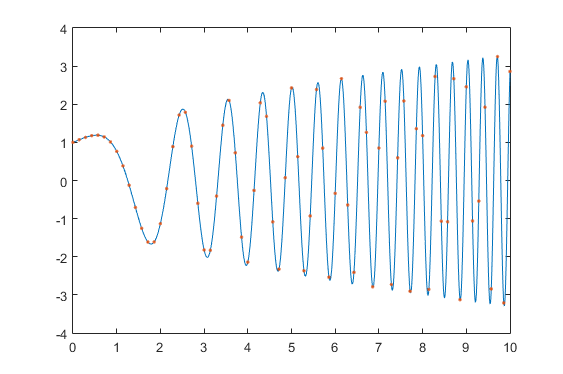
\includegraphics[scale=1]{nastyProb.png}
\end{figure}

After we have a simulator instance, the user can configure some parameters and ask the simulator to solve the system using PSM. The above codes use PSM method to calculate value from 0 to 20, and plot the result. As we can see, all the red dots (the correct answer) follow on the estimation (blue line). The PSM method successfully calculate the complex function.

\clearpage
\subsection{sin(t)}

\begin{equation}
\mathscr{L}^{-1}\{\frac{1}{s^2 + 1}\} = \sin(t) \quad\scriptscriptstyle
\end{equation}

The second example, we will illustrate how our program inverse Laplace transform. First of all, let's normalize the system and get the following simple form.
\begin{equation}
x(t) = \frac{1}{t^2 + 1} \quad x'(t) = \frac{2t}{(t^2 + 1)^2} = 2t *x(t)^2
\end{equation}
This system is then supplied into the system represented in the format illustrate in the previous section.
\begin{lstlisting}
s = simulator( {@(s)1/(s^2+1)} , 0 , ...
   [rel(1,-2, 1, [1 1]) ] );
   
%% convergence
figure(1)
hold off
t = 5;
kk = 1 : 100 : 1000;
answer = sin(t);
vv = s.converge( t , kk);
plot(kk , vv ,'-', kk , ones(1, size(kk,2)) * answer , '.');

%% inverseTransform
figure(4)
hold off
tt = 0 : 1 : 20;
k = @(t) t .^3 + 100;
answer = @(t) sin(t);
vv = s.converge( tt, ceil(k(tt)));
plot(tt, vv ,'-', tt, answer(tt), '.');

figure(5)
plot(tt, vv - answer(tt) ,'-');
\end{lstlisting}

s.converge(t, k) compute $v(t, k)$, given value of t and k. If either or both of t and k is an array, an array of results will be returned.
\begin{equation*}
v(t, k) = \frac{(-1)^{k}}{k!} \left(\frac{k}{t}\right)^{k+1}  F^{(k)} \left(\frac{k}{t}\right)
\end{equation*}
The convergence section plot how v(t,k) converges to the inverse Laplace transform.

The inverseTransform section plot the actual Inverse Laplace transform. This example takes 17sec to compute.
The following table summarize the v(t,k), error and time to compute. As we can see, as t grows, it takes longer for v(t,k) to converge and needs larger k and longer time.

\begin{tabular}{| l | l | l | l | l | l |}
\hline
t  &  k   &  [v(t,k)] & [sin(t)] & error & time \\
\hline
1  &  100 &  0.8425 & 0.8415 & 0.001077 & 0.042 \\
\hline
1  &  1000 &  0.8416 & 0.8415 & 1.1838e-04 & 0.214 \\
\hline
1  &  10000 &  0.8415 & 0.8415 & 1.2057e-05 & 2.536 \\
\hline
10  &  100 &  -0.3622 & -0.5440 & 0.1819 & 0.070 \\
\hline
10  &  1000 &  -0.5252 & -0.5440 & 0.0189 & 0.209 \\
\hline
10  &  10000 &  -0.5421 & -0.5440 & 0.0019 & 2.566 \\
\hline
10  &  100000 &  -0.5438 & -0.5440 & 1.8907e-04 & 176.150\\
\hline
100  &  100 &  -4.4409e-16 & -0.5064 & 0.5064 & 0.072 \\
\hline
100  &  1000 &  -0.0047 & -0.5064 & 0.5016 & 0.072 \\
\hline
100  &  10000 &  -0.3036 & 0.2027 & 0.2027 & 2.673 \\
\hline
100  &  100000 &  -0.4809 & 0.2027 & 0.0255 & 148.276  \\
\hline
\end{tabular}

https://github.com/fredzqm/NumericInverseLaplace/blob/master/

\clearpage
\begin{thebibliography}{99}
\bibitem{KB} Kurt Bryan. {\it Elementary Inversion of the Laplace Transform} https://www.rose-hulman.edu/~bryan/invlap.pdf

\bibitem{OV} G.E. Parker, J.S. Sochacki et al., An Overview of the Modied Picard
Method, http://educ.jmu.edu/sochacjs/expository.pdf

\bibitem{CL} E.A. Coddington and N. Levinson, Theory of Ordinary Differential Equations, McGraw-Hill, New York, 1955

\bibitem{PS} G.E. Parker and J.S. Sochacki, Implementing the Picard Iteration, Neural, Parallel and Scientic Computations, 4 (1996) 1, pp. 97-112.

\bibitem{CPSW} D.C. Carothers, G.E. Parker, J.S. Sochacki and P. G. Warne, Some
Properties of Solutions to Polynomial Systems of Equations, Elec. Jour. of Diff. Eqn.,
2005 (2005) 40, pp. 1-17.

\bibitem{EX} P. G. Warne, D. A. P. Warne, J. S. Sochacki, G. E. Parker and D. C.
Carothers, Explicit A-Priori Error Bounds and Adaptive Error Control for Approx-
imation of Nonlinear Initial Value Differential Systems, Comput. Math. Appl., 52
(2006), pp. 1695-1710.

\bibitem{PSM} Kurt Bryan. {\it Elementary Inversion of the Laplace Transform} https://www.rose-hulman.edu/~bryan/invlap.pdf

\bibitem{NORMAL} Kurt Bryan. {\it Elementary Inversion of the Laplace Transform} https://www.rose-hulman.edu/~bryan/invlap.pdf

\bibitem{SETTLE} Kurt Bryan. {\it Elementary Inversion of the Laplace Transform} https://www.rose-hulman.edu/~bryan/invlap.pdf

\bibitem{BE} Kurt Bryan. {\it Elementary Inversion of the Laplace Transform} https://www.rose-hulman.edu/~bryan/invlap.pdf

\end{thebibliography}

\end{document}